\chapter{Refleks Regang dan Pesan Saraf}\label{ch:g12:stretch-reflex}

Seorang dokter mengetuk \omterm{def:g10:muscles-and-joints:muscle}{tendon} tepat di bawah tempurung lututmu dengan
sebuah palu karet kecil, dan kakimu menendang ke depan sebelum kamu
merasakan apa pun. Tiga puluh milidetik memisahkan ketukan dari
tendangannya: terlalu singkat bagi otak, bahkan terlalu singkat bagi
sebuah keputusan. Isyaratnya pergi dari otot ke sumsum tulang belakang
lalu kembali --- sebuah sirkuit berisi dua \omterm{def:g12:stretch-reflex:neuron}{neuron} dan satu sambungan di
antaranya --- dan sirkuit yang sama itulah yang menjagamu tegak,
diam-diam, setiap detik kamu berdiri. Bab ini memakainya untuk
memperkenalkan \omterm{def:g12:stretch-reflex:neuron}{neuron}, isyarat listrik yang dibawanya, dan sambungan
kimia tempat satu \omterm{def:g12:stretch-reflex:neuron}{neuron} berbicara kepada \omterm{def:g12:stretch-reflex:neuron}{neuron} berikutnya.

\section{Lengkung refleks}

\begin{definition}[Refleks]\label{def:g12:stretch-reflex:reflex}
Sebuah \emph{refleks}\index{refleks} adalah tanggapan sebuah efektor
(sebuah otot atau sebuah kelenjar) yang tak disengaja, cepat dan
berpola tetap terhadap sebuah rangsangan, yang dihasilkan oleh sirkuit
\omterm{def:g12:stretch-reflex:neuron}{neuron} yang tetap, yaitu \emph{lengkung refleks}\index{lengkung
refleks}, yang berjalan lewat sumsum tulang belakang atau batang otak
tanpa memerlukan otak. \emph{Refleks regang}\index{refleks regang}
adalah yang paling sederhana: peregangan mendadak sebuah otot membuat
otot itu sendiri berkontraksi.
\end{definition}

\begin{proposition}[Sirkuit refleks regang]\label{prop:g12:stretch-reflex:arc}
Lima unsur, menurut urutannya:
\begin{enumerate}
  \item \emph{reseptornya}: \emph{kumparan otot}, yaitu organ indra
        kecil yang terletak di antara \omterm{def:g10:muscles-and-joints:muscle}{serat otot}, yang ikut teregang
        ketika ototnya teregang lalu menanggapinya dengan melepaskan
        isyarat;
  \item \emph{\omterm{def:g12:stretch-reflex:neuron}{neuron} sensorik}, yang seratnya berjalan dari kumparan
        itu ke sumsum tulang belakang, masuk lewat akar dorsal; badan
        \omterm{def:g10:cells-common-unit:cell}{selnya} terletak di sebuah ganglion di samping sumsumnya;
  \item \emph{pusat pemaduan}: materi kelabu sumsum tulang belakang,
        tempat serat sensoriknya bersambung langsung --- lewat satu
        \omterm{def:g12:stretch-reflex:synapse}{sinapsis} tunggal --- ke \omterm{def:g12:stretch-reflex:neuron}{neuron} motorik otot yang sama, dan,
        lewat sebuah \omterm{def:g12:stretch-reflex:neuron}{neuron} perantara, menghambat \omterm{def:g12:stretch-reflex:neuron}{neuron} motorik otot
        antagonisnya;
  \item \emph{\omterm{def:g12:stretch-reflex:neuron}{neuron} motorik}, yang seratnya keluar lewat akar ventral
        lalu berjalan ke ototnya;
  \item \emph{efektornya}: \omterm{def:g10:muscles-and-joints:muscle}{serat otot}, yang berkontraksi.
\end{enumerate}
Sebuah ketukan pada \omterm{def:g10:muscles-and-joints:muscle}{tendon} patela meregangkan otot pahanya; kumparannya
melepaskan isyarat; \omterm{def:g12:stretch-reflex:neuron}{neuron} motorik otot itu melepaskan isyarat;
ototnya berkontraksi dan tungkainya menjulur, sementara otot paha
belakangnya disuruh mengendur.
\end{proposition}
\begin{proof}[Bukti percobaan]
Memotong akar dorsal melenyapkan \omterm{def:g12:stretch-reflex:reflex}{refleksnya} sedangkan ototnya masih
dapat dibuat berkontraksi dengan merangsang akar ventralnya; memotong
akar ventral melenyapkannya sedangkan serat sensoriknya masih membawa
isyarat ketika ototnya diregangkan: lengkungnya punya pintu masuk
sensorik dan pintu keluar motorik. \omterm{def:g12:stretch-reflex:reflex}{Refleksnya} bertahan pada hewan yang
sumsum tulang belakangnya diputus dari otaknya: otaknya tidak
diperlukan. Perekaman dari serat tunggal menunjukkan isyarat
kumparannya mulai dalam waktu semilidetik setelah peregangannya, dan
\omterm{def:g12:stretch-reflex:neuron}{neuron} motoriknya melepaskan isyarat sekitar semilidetik setelah
isyarat sensoriknya tiba --- yaitu tundaan satu \omterm{def:g12:stretch-reflex:synapse}{sinapsis}.
\end{proof}

\begin{omfigure}
\begin{tikzpicture}[font=\small, >=Stealth, line cap=round]
  % spinal cord section (simplified): outer white, inner grey H
  \draw[thick, fill=omDef!6] (0,0) ellipse (2.2 and 1.5);
  \draw[thick, fill=gray!25] (-0.9,-1.0) -- (-0.9,0.3) .. controls (-0.9,0.9) .. (-0.5,1.0) -- (-0.3,0.4) -- (0.3,0.4) -- (0.5,1.0) .. controls (0.9,0.9) .. (0.9,0.3) -- (0.9,-1.0) .. controls (0.6,-1.1) .. (0.3,-0.5) -- (-0.3,-0.5) .. controls (-0.6,-1.1) .. (-0.9,-1.0) -- cycle;
  \node[font=\scriptsize] at (0,-1.25) {materi kelabu};
  \node[anchor=south, font=\scriptsize] at (0,1.6) {sumsum tulang belakang (irisan)};
  % sensory neuron: from spindle (right, muscle) to dorsal root (top right) into grey matter
  \draw[thick, omDef] (5.4,1.2) -- (3.2,1.2) -- (2.4,1.1);
  \draw[thick, omDef] (2.4,1.1) .. controls (1.4,0.9) .. (0.55,0.5);
  \fill[omDef] (2.7,1.2) circle (3pt); \node[font=\scriptsize, omDef, anchor=south] at (2.7,1.35) {badan sel};
  \node[font=\scriptsize, omDef, anchor=south] at (4.4,1.3) {neuron sensorik};
  % motor neuron: cell body in ventral grey, axon out ventral root to muscle
  \fill[omThm] (0.55,-0.7) circle (4pt);
  \draw[thick, omThm] (0.55,-0.7) .. controls (1.6,-1.2) .. (2.6,-1.3) -- (5.4,-1.3);
  \node[font=\scriptsize, omThm, anchor=north] at (4.2,-1.4) {neuron motorik};
  % synapse mark
  \fill[omProp] (0.55,0.5) circle (2pt); \draw[omProp, thick] (0.55,0.45) -- (0.55,-0.6);
  \node[font=\scriptsize, omProp, anchor=west] at (1.0,-0.15) {sinapsis};
  % interneuron to antagonist
  \fill[omMeth!70!black] (-0.5,-0.2) circle (3pt);
  \draw[thick, omMeth!70!black] (0.5,0.5) .. controls (0.0,0.4) .. (-0.5,-0.2);
  \draw[thick, omMeth!70!black, dashed] (-0.5,-0.2) .. controls (-1.3,-0.9) .. (-2.4,-1.2) -- (-3.2,-1.2);
  \node[font=\scriptsize, omMeth!70!black, anchor=north, align=center] at (-2.4,-1.35) {menghambat neuron motorik\\ otot antagonisnya};
  % muscle with spindle (right)
  \draw[thick, fill=omThm!25, rounded corners=8pt] (5.4,-1.7) rectangle (7.6,1.7);
  \node[font=\scriptsize] at (6.5,-1.4) {otot};
  \draw[thick, fill=omDef!30] (6.5,1.2) ellipse (0.55 and 0.25);
  \node[font=\scriptsize] at (6.5,0.7) {kumparan otot};
  \draw[->, thick] (6.5,2.75) -- (6.5,1.85) node[pos=0, above, align=center, font=\scriptsize] {ketukan pada tendon:\\ ototnya teregang};
  \node[font=\scriptsize, anchor=north, align=center] at (6.5,-1.85) {serat motorik berakhir pada\\ ototnya: kontraksi};
\end{tikzpicture}

{\small \omterm{def:g12:stretch-reflex:reflex}{Lengkung refleks} regang, dilihat pada irisan sumsum tulang
belakang. \omterm{def:g12:stretch-reflex:neuron}{Neuron} sensorik kumparannya (biru) masuk lewat akar dorsal
lalu bersambung, melalui satu \omterm{def:g12:stretch-reflex:synapse}{sinapsis} (jingga), ke \omterm{def:g12:stretch-reflex:neuron}{neuron} motorik
(merah) otot yang sama, yang keluar lewat akar ventral; sebuah
interneuron (hijau) menghambat antagonisnya.}
\end{omfigure}

\begin{omfigure}

\includegraphics[width=0.56\linewidth]{images/book2/ai/g12-reflex-hammer.jpg}

{\small Uji sentakan lutut: sebuah ketukan pada \omterm{def:g10:muscles-and-joints:muscle}{tendon} patela
meregangkan otot pahanya, dan tiga puluh milidetik kemudian tungkainya
menendang. \omterm{def:g12:stretch-reflex:reflex}{Refleks} itu memeriksa, dalam sedetik, seluruh lengkungnya
dari kumparan sampai otot.}
\end{omfigure}

\begin{example}[Untuk apa refleks itu]\label{ex:g12:stretch-reflex:posture}
Ketika berdiri, kamu berayun; tiap ayunan meregangkan otot pada satu
sisi pergelangan kaki, yang kumparannya melepaskan isyarat dan yang
kontraksi \omterm{def:g12:stretch-reflex:reflex}{refleksnya} menarikmu kembali sebelum kamu menyadarinya.
Ketika membawa nampan, tambahan berat yang mendadak meregangkan otot
lenganmu dan \omterm{def:g12:stretch-reflex:reflex}{refleksnya} mengakukan otot itu dalam \qty{30}{ms}, sebelum
nampannya tumpah. \omterm{def:g12:stretch-reflex:reflex}{Refleks regang} adalah sebuah servomekanisme: ia
melawan setiap perubahan panjang sebuah otot, dan otak menyetel
kepekaannya untuk menetapkan tonus tubuh --- lebih tinggi ketika kamu
bersiaga, lebih rendah ketika kamu tidur.
\end{example}

\section{Neuron dan pesannya}

\begin{definition}[Neuron]\label{def:g12:stretch-reflex:neuron}
Sebuah \emph{neuron}\index{neuron} adalah \omterm{def:g10:cells-common-unit:cell}{sel} yang dikhususkan untuk
mengisyaratkan: sebuah badan \omterm{def:g10:cells-common-unit:cell}{sel} dengan intinya, \emph{dendrit} yang
bercabang untuk menerima isyarat, dan satu serat panjang tunggal, yaitu
\emph{akson}, yang membawa isyarat neuron itu sendiri ke ujungnya ---
bagi neuron motorik tungkai, sejauh satu meter. Banyak akson terbungkus
selubung berlemak, yaitu \emph{mielin}, yang dibentuk \omterm{def:g10:cells-common-unit:cell}{sel} pendamping,
dan yang mempercepat penghantarannya. Sebuah saraf adalah seberkas
ratusan atau ribuan akson.
\end{definition}

\begin{omfigure}
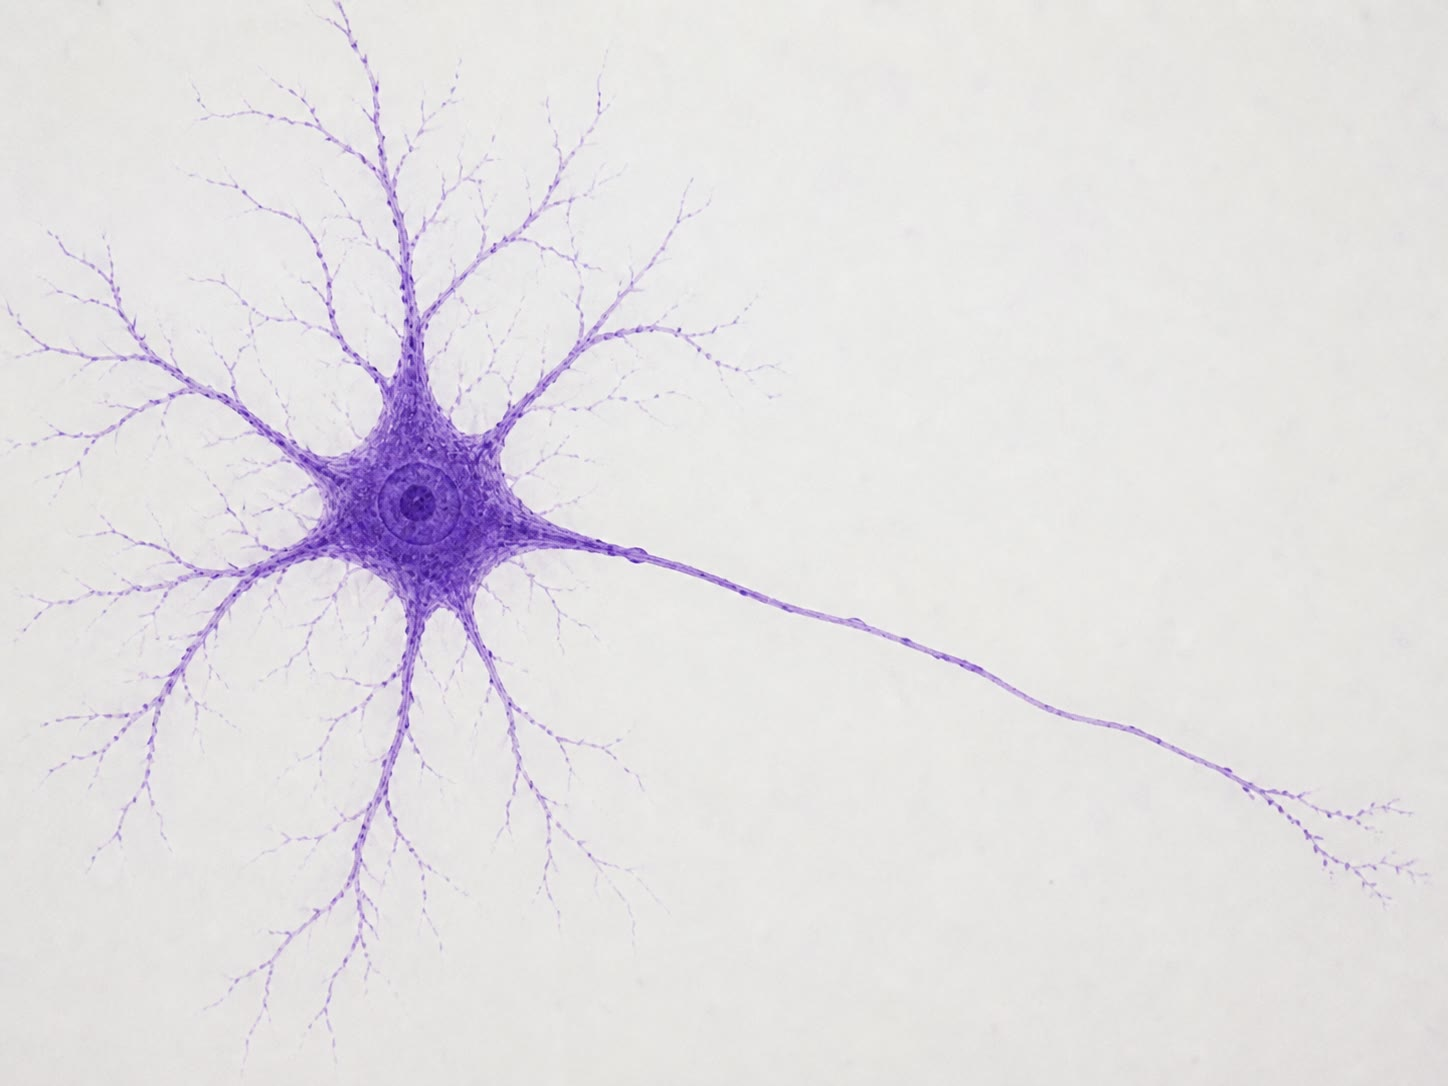
\includegraphics[width=0.5\linewidth]{images/book2/ai/g12-neuron-micrograph.jpg}

{\small Sebuah \omterm{def:g12:stretch-reflex:neuron}{neuron} motorik yang diwarnai: badan \omterm{def:g10:cells-common-unit:cell}{selnya} dengan
intinya, dendrit bercabang yang menerima isyarat, dan akson tunggal
yang keluar membawa pesan \omterm{def:g12:stretch-reflex:neuron}{neuron} itu sendiri ke sebuah otot.}
\end{omfigure}

\begin{proposition}[Potensial aksi]\label{prop:g12:stretch-reflex:actionpotential}
Membran sebuah \omterm{def:g12:stretch-reflex:neuron}{neuron} memuat tegangan listrik: bagian dalamnya sekitar
\qty{-70}{mV} terhadap bagian luarnya saat istirahat. \emph{Pesan
saraf}\index{pesan saraf} adalah sederet \emph{potensial
aksi}\index{potensial aksi}: pembalikan singkat tegangan itu, yang
masing-masing naik sampai sekitar \qty{+30}{mV} dan kembali dalam
semilidetik, dan yang berjalan sepanjang aksonnya tanpa melemah.
Sebuah \omterm{prop:g12:stretch-reflex:actionpotential}{potensial aksi} bersifat \emph{semua atau tak sama sekali}:
rangsangan di bawah sebuah ambang tak menghasilkan apa-apa, dan
rangsangan mana pun di atasnya menghasilkan isyarat berukuran penuh
yang sama. Karena itu kuatnya sebuah rangsangan tersandi bukan pada
besar isyaratnya melainkan pada \emph{frekuensinya}: regangan yang
lebih kuat membuat kumparannya melepaskan lebih banyak \omterm{prop:g12:stretch-reflex:actionpotential}{potensial aksi}
tiap detik.
\end{proposition}
\begin{proof}[Bukti percobaan]
Mikroelektrode yang ditusukkan ke dalam sebuah akson merekam tegangan
istirahatnya dan, ketika \omterm{def:g10:cells-common-unit:cell}{selnya} melepaskan isyarat, paku yang identik
yang bentuknya tak berubah oleh rangsangannya maupun oleh jarak yang
ditempuhnya. Perekaman dari serat kumparan tunggal selama regangan yang
makin kuat menunjukkan paku berukuran tetap dengan laju yang naik dari
beberapa sampai beberapa ratus tiap detik. Rangsangan yang tepat di
bawah ambangnya sama sekali tak memberi paku; melipatduakan rangsangan
yang sudah di atas ambangnya mengubah lajunya, tak pernah tingginya.
\end{proof}

\begin{omfigure}
\begin{tikzpicture}
\begin{axis}[
  width=0.62\linewidth, height=5.6cm,
  axis x line=bottom, axis y line=left,
  xmin=0, xmax=5, ymin=-100, ymax=50,
  xlabel={waktu (ms)}, ylabel={tegangan membran (mV)},
  xlabel style={font=\small, at={(axis description cs:0.5,-0.12)}, anchor=north},
  ylabel style={font=\small},
  tick label style={font=\small}, xtick={0,1,2,3,4,5}, ytick={-70,-30,0,30},
  clip=false,
]
\addplot[thick, omThm, smooth] coordinates {(0,-70) (1,-70) (1.3,-55) (1.5,-20) (1.7,30) (1.9,10) (2.1,-40) (2.3,-75) (2.7,-80) (3.2,-72) (4,-70) (5,-70)};
\draw[dashed, gray] (axis cs:0,-55) -- (axis cs:5,-55);
\node[font=\scriptsize, gray, anchor=south west] at (axis cs:3.3,-55) {ambang};
\node[font=\scriptsize, anchor=south west] at (axis cs:0.1,-68) {istirahat};
\node[font=\scriptsize, anchor=west] at (axis cs:1.8,32) {puncak};
\end{axis}
\end{tikzpicture}

{\small Sebuah \omterm{prop:g12:stretch-reflex:actionpotential}{potensial aksi} yang direkam di dalam sebuah akson: dari
\qty{-70}{mV} saat istirahat, naik cepat melewati ambangnya sampai
sekitar \qty{+30}{mV}, kembali di bawah taraf istirahatnya, lalu pulih
--- semuanya dalam sekitar dua milidetik. Setiap \omterm{prop:g12:stretch-reflex:actionpotential}{potensial aksi} sebuah
\omterm{def:g12:stretch-reflex:neuron}{neuron} tertentu berbentuk sama.}
\end{omfigure}

\begin{omfigure}
\begin{tikzpicture}[font=\small, line cap=round]
  \foreach \row/\y/\lab/\n in {1/2.4/{regangan lemah}/6, 2/1.2/{regangan sedang}/12, 3/0/{regangan kuat}/24} {
    \draw[thick] (0,\y) -- (9,\y);
    \node[anchor=east] at (-0.2,\y) {\lab};
  }
  \foreach \i in {1,...,6} \draw[very thick, omThm] ({\i*9/7},2.4) -- ({\i*9/7},2.4+0.6);
  \foreach \i in {1,...,12} \draw[very thick, omThm] ({\i*9/13},1.2) -- ({\i*9/13},1.2+0.6);
  \foreach \i in {1,...,24} \draw[very thick, omThm] ({\i*9/25},0) -- ({\i*9/25},0.6);
  \draw[<->] (0,-0.5) -- (9,-0.5) node[midway, below] {\qty{100}{ms}};
\end{tikzpicture}

{\small Penyandian frekuensi. Serat kumparan yang sama direkam selama
tiga regangan: pakunya identik, dan hanya lajunya yang berubah ---
sekitar 60, 120 dan 240 tiap detik di sini.}
\end{omfigure}

\begin{example}[Kelajuan]\label{ex:g12:stretch-reflex:speed}
\omterm{prop:g12:stretch-reflex:actionpotential}{Potensial aksi} berjalan \qty{1}{m/s} pada serat tipis tanpa mielin dan
sampai \qty{100}{m/s} pada serat tebal bermielin milik \omterm{def:g12:stretch-reflex:reflex}{refleks regang}.
Dari lutut ke sumsum tulang belakang lalu kembali kira-kira
\qty{1.5}{m}: sekitar \qty{15}{ms} perjalanan, yang ditambah lagi
\qty{15}{ms} oleh tanggapan kumparannya, satu \omterm{def:g12:stretch-reflex:synapse}{sinapsis} dan pengaktifan
ototnya --- itulah \qty{30}{ms} sentakan lutut. Pesan dari sebuah jari
kaki ke otak, sejauh \qty{1.8}{m}, memakan sekitar \qty{20}{ms};
keputusan untuk menggerakkannya, dan pelaksanaannya, sekitar
\qty{150}{ms} lagi.
\end{example}

\section{Sinapsis}

\begin{definition}[Sinapsis dan neurotransmiter]\label{def:g12:stretch-reflex:synapse}
Sebuah \emph{sinapsis}\index{sinapsis} adalah sambungan tempat ujung
akson satu \omterm{def:g12:stretch-reflex:neuron}{neuron} bertemu \omterm{def:g10:cells-common-unit:cell}{sel} berikutnya --- sebuah \omterm{def:g12:stretch-reflex:neuron}{neuron} atau sebuah
\omterm{def:g10:muscles-and-joints:muscle}{serat otot} --- menyeberangi celah selebar sekitar \qty{20}{nm}, yaitu
\emph{celah sinapsis}. Isyaratnya tidak melompati celah itu secara
listrik: \omterm{prop:g12:stretch-reflex:actionpotential}{potensial aksi} yang tiba membuat ujungnya melepaskan, dari
vesikel kecil, sebuah pembawa pesan kimia, yaitu
\emph{neurotransmiter}\index{neurotransmiter}, ke dalam celahnya;
neurotransmiter itu mengikat \emph{reseptor} pada membran \omterm{def:g10:cells-common-unit:cell}{sel}
penerimanya, yang lalu mengubah tegangan \omterm{def:g10:cells-common-unit:cell}{sel} itu; ia kemudian
dihancurkan atau ditarik kembali dalam beberapa milidetik. Sinapsis
mengubah pesan listrik menjadi pesan kimia lalu kembali lagi, dan
banyaknya transmiter yang dilepaskan --- yang ditetapkan oleh frekuensi
\omterm{prop:g12:stretch-reflex:actionpotential}{potensial aksi} yang tiba --- menyandikan kuatnya pesan itu.
\end{definition}

\begin{omfigure}
\begin{tikzpicture}[font=\small, >=Stealth, line cap=round]
  % presynaptic ending
  \draw[thick, fill=omDef!12] (0,0) -- (3.0,0) .. controls (4.0,0) and (4.0,2.6) .. (3.0,2.6) -- (0,2.6);
  \node[anchor=east, align=right, omDef!80!black] at (-0.1,1.3) {ujung akson\\ (potensial aksi\\ berdatangan)};
  \foreach \x/\y in {2.2/0.7, 2.6/1.3, 2.3/1.9, 1.6/1.2, 3.1/1.0, 3.1/1.7} \draw[thick, fill=omThm!25] (\x,\y) circle (0.22);
  \node[font=\scriptsize, anchor=south] at (1.6,1.5) {vesikel};
  % cleft
  \draw[thick, fill=omDef!12] (4.6,-0.4) -- (4.6,3.0) -- (8.5,3.0) -- (8.5,-0.4) -- cycle;
  \node[anchor=west, align=left, omMeth!70!black] at (5.0,2.45) {sel penerima\\ (neuron atau otot)};
  \foreach \y in {0.5,1.1,1.7} \draw[thick, fill=omMeth!40] (4.5,\y-0.15) rectangle (4.85,\y+0.15);
  \node[font=\scriptsize, anchor=west] at (5.0,1.1) {reseptor};
  % transmitter molecules in cleft
  \foreach \x/\y in {4.05/0.6, 4.25/1.2, 4.1/1.6, 4.3/0.9, 4.2/1.9} \fill[omThm] (\x,\y) circle (2pt);
  \node[font=\scriptsize, anchor=north, align=center] at (4.25,-0.55) {celah: transmiter\\ dilepaskan, lalu dihancurkan};
  \draw[->, thick] (3.35,1.3) -- (3.95,1.3);
  \draw[->, thick] (4.95,2.1) .. controls (5.6,2.0) .. (6.3,1.5) node[right, font=\scriptsize] {tegangannya berubah};
\end{tikzpicture}

{\small Sebuah \omterm{def:g12:stretch-reflex:synapse}{sinapsis}. \omterm{prop:g12:stretch-reflex:actionpotential}{Potensial aksi} yang mencapai ujungnya membuat
vesikel melepaskan \omterm{def:g12:stretch-reflex:synapse}{neurotransmiter} ke dalam celahnya; transmiter itu
mengikat reseptor pada \omterm{def:g10:cells-common-unit:cell}{sel} penerima lalu mengubah tegangannya; \omterm{def:g11:enzymes-and-phenotype:enzyme}{enzim}
kemudian menghancurkannya. Pesannya menyeberang sebagai zat kimia,
hanya ke satu arah.}
\end{omfigure}

\begin{proposition}[Eksitasi, inhibisi, dan sambungan ototnya]\label{prop:g12:stretch-reflex:junction}
Bergantung pada transmiternya dan reseptornya, sebuah \omterm{def:g12:stretch-reflex:synapse}{sinapsis}
\emph{merangsang} \omterm{def:g12:stretch-reflex:neuron}{neuron} penerimanya (membawanya menuju ambangnya)
atau \emph{menghambatnya} (menjauhkannya). \omterm{def:g12:stretch-reflex:reflex}{Refleks regang} memakai
keduanya: perangsangan \omterm{def:g12:stretch-reflex:neuron}{neuron} motorik otot itu sendiri, dan penghambatan
\omterm{def:g12:stretch-reflex:neuron}{neuron} motorik antagonisnya lewat interneuron. Pada \emph{sambungan
neuromuskular}, yaitu \omterm{def:g12:stretch-reflex:synapse}{sinapsis} antara sebuah \omterm{def:g12:stretch-reflex:neuron}{neuron} motorik dan sebuah
\omterm{def:g10:muscles-and-joints:muscle}{serat otot}, transmiternya adalah \emph{asetilkolina}: tiap \omterm{prop:g12:stretch-reflex:actionpotential}{potensial
aksi} \omterm{def:g12:stretch-reflex:neuron}{neuron} motorik melepaskannya cukup banyak untuk memicu seratnya,
yang lalu berkontraksi. Sebuah \omterm{def:g12:stretch-reflex:neuron}{neuron} motorik dan serat yang
diperintahnya membentuk sebuah \emph{unit motorik}; gaya sebuah otot
ditetapkan oleh berapa banyak unit yang memicu dan seberapa cepat.
\end{proposition}
\begin{proof}[Bukti percobaan]
Asetilkolina yang diterapkan pada sebuah \omterm{def:g10:muscles-and-joints:muscle}{serat otot} membuatnya
berkontraksi; \emph{kurare}, racun panah itu, mengikat reseptor
asetilkolina seratnya tanpa mengaktifkannya lalu melumpuhkan setiap
otot sementara sarafnya terus melepaskan isyarat; toksin botulisme
menghambat pelepasan vesikelnya dan melumpuhkan dengan cara serupa;
sebuah insektisida yang menghambat \omterm{def:g11:enzymes-and-phenotype:enzyme}{enzim} penghancur asetilkolina
membuat ototnya berkontraksi tanpa kendali. Striknina menghambat
\omterm{def:g12:stretch-reflex:synapse}{sinapsis} penghambat sumsum tulang belakang, sehingga tiap regangan
memicu kontraksi ototnya sekaligus antagonisnya: kejang. Tiap racun itu
menamai sebuah langkah sambungannya dengan menyingkirkannya.
\end{proof}

\begin{method}[Menganalisis sebuah refleks atau sebuah racun]\label{met:g12:stretch-reflex:analyse}
\begin{enumerate}
  \item Lacaklah lengkungnya: reseptor, \omterm{def:g12:stretch-reflex:neuron}{neuron} sensorik, pusat, \omterm{def:g12:stretch-reflex:neuron}{neuron}
        motorik, efektor; kenali unsur mana yang dikenai sebuah lesi
        atau sebuah obat.
  \item Pada tiap \omterm{def:g12:stretch-reflex:neuron}{neuron}, tanyakan apa yang tersandi --- yaitu
        frekuensi \omterm{prop:g12:stretch-reflex:actionpotential}{potensial aksinya} --- dan pada tiap \omterm{def:g12:stretch-reflex:synapse}{sinapsis}, apa
        yang membawa pesannya --- yaitu transmiternya dan jumlahnya.
  \item Untuk sebuah racun, temukan langkahnya: pelepasan transmiternya,
        reseptornya, penghancuran transmiternya, atau sebuah \omterm{def:g12:stretch-reflex:synapse}{sinapsis}
        penghambat; ramalkan kelumpuhan (tak ada yang lolos) atau
        kejang (tak ada yang dihentikan).
  \item Hitunglah waktunya: jarak dibagi kelajuan penghantaran, ditambah
        sekitar semilidetik tiap \omterm{def:g12:stretch-reflex:synapse}{sinapsis}.
\end{enumerate}
\end{method}

\begin{remark}[Sebuah pesan yang tersusun dari paku yang sama]\label{rem:g12:stretch-reflex:spikes}
Setiap pesan di dalam sistem saraf --- regangan kumparannya, cahaya
retinanya, perintah otak untuk bergerak --- tersusun dari \omterm{prop:g12:stretch-reflex:actionpotential}{potensial
aksi} semua-atau-tak-sama-sekali yang sama, yang berbeda hanya pada
lajunya dan pada kabel yang membawanya; maknanya terletak pada \omterm{def:g12:stretch-reflex:neuron}{neuron}
mana yang melepaskan isyarat, bukan pada apa yang dilepaskannya. Dan
pada setiap \omterm{def:g12:stretch-reflex:synapse}{sinapsis} pesan itu menjadi sedosis zat kimia, dan itulah
sebabnya sebuah molekul --- sebuah transmiter, sebuah racun, sebuah
obat --- dapat masuk ke percakapannya di titik mana pun. Bab terakhir
mengikuti paku dan \omterm{def:g12:stretch-reflex:synapse}{sinapsis} yang sama itu naik ke dalam otak, dan
perintah yang turun kembali.
\end{remark}

\section{Latihan}

\begin{exercise}[$\star$]\label{exo:g12:stretch-reflex:1}
Sebutkan kelima unsur \omterm{def:g12:stretch-reflex:reflex}{lengkung refleks} regang, menurut urutannya.
\end{exercise}

\begin{exercise}[$\star$]\label{exo:g12:stretch-reflex:2}
Uraikan bagian sebuah \omterm{def:g12:stretch-reflex:neuron}{neuron} dan arah perjalanan pesannya.
\end{exercise}

\begin{exercise}[$\star$]\label{exo:g12:stretch-reflex:3}
Apa itu \omterm{prop:g12:stretch-reflex:actionpotential}{potensial aksi}? Apa arti ``semua atau tak sama sekali'', dan
bagaimana kuatnya rangsangan tersandi?
\end{exercise}

\begin{exercise}[$\star$]\label{exo:g12:stretch-reflex:4}
Uraikan peristiwa pada sebuah \omterm{def:g12:stretch-reflex:synapse}{sinapsis}, dari tibanya \omterm{prop:g12:stretch-reflex:actionpotential}{potensial aksi}
sampai tanggapan \omterm{def:g10:cells-common-unit:cell}{sel} penerimanya.
\end{exercise}

\begin{exercise}[$\star$]\label{exo:g12:stretch-reflex:5}
Transmiter mana yang bekerja pada sambungan neuromuskular, dan apa yang
dilakukan kurare serta toksin botulinum terhadapnya?
\end{exercise}

\begin{exercise}[$\star\star$]\label{exo:g12:stretch-reflex:6}
Dari gambar penyandian frekuensi, cacahlah pakunya dalam \qty{100}{ms}
bagi tiap regangan lalu sebutkan lajunya. Apa yang tidak berubah antara
barisnya?
\end{exercise}

\begin{exercise}[$\star\star$]\label{exo:g12:stretch-reflex:7}
Waktu tunda sentakan lutut \qty{30}{ms} untuk lintasan sepanjang
\qty{1.5}{m}. Jika \omterm{def:g12:stretch-reflex:synapse}{sinapsis} dan pengaktifan ototnya bersama-sama
memakan \qty{12}{ms}, hitunglah kelajuan penghantaran seratnya.
\end{exercise}

\begin{exercise}[$\star\star$]\label{exo:g12:stretch-reflex:8}
Jelaskan mengapa memotong akar dorsal melenyapkan \omterm{def:g12:stretch-reflex:reflex}{refleksnya} tetapi
tidak kesanggupan ototnya berkontraksi, sedangkan memotong akar ventral
melenyapkan keduanya.
\end{exercise}

\begin{exercise}[$\star\star$]\label{exo:g12:stretch-reflex:9}
Mengapa otot antagonisnya harus dihambat selama \omterm{def:g12:stretch-reflex:reflex}{refleksnya}? Unsur mana
pada lengkungnya yang melakukannya, dan lewat \omterm{def:g12:stretch-reflex:synapse}{sinapsis} macam apa?
\end{exercise}

\begin{exercise}[$\star\star$]\label{exo:g12:stretch-reflex:10}
Sebuah rangsangan sebesar 2 satuan tepat berada pada ambang sebuah
\omterm{def:g12:stretch-reflex:neuron}{neuron} dan memberi satu \omterm{prop:g12:stretch-reflex:actionpotential}{potensial aksi} sebesar \qty{100}{mV}. Ramalkan
isyarat bagi rangsangan sebesar 1, 4 dan 8 satuan.
\end{exercise}

\begin{exercise}[$\star\star$]\label{exo:g12:stretch-reflex:11}
Jelaskan mengapa pesannya menyeberangi sebuah \omterm{def:g12:stretch-reflex:synapse}{sinapsis} hanya ke satu
arah, dan mengapa pesan itu tertunda di sana sekitar semilidetik.
\end{exercise}

\begin{exercise}[$\star\star\star$]\label{exo:g12:stretch-reflex:12}
Sebuah insektisida menghambat \omterm{def:g11:enzymes-and-phenotype:enzyme}{enzim} penghancur asetilkolina. Ramalkan
pengaruhnya pada sambungan neuromuskular dan pada pernapasan, lalu
jelaskan mengapa obat yang menghambat reseptor asetilkolina dipakai
sebagai penawar pada dosis yang diukur cermat.
\end{exercise}

\begin{exercise}[$\star\star\star$]\label{exo:g12:stretch-reflex:13}
Striknina menghambat \omterm{def:g12:stretch-reflex:synapse}{sinapsis} penghambat di sumsum tulang belakang.
Dengan memakai \omterm{def:g12:stretch-reflex:reflex}{lengkung refleksnya}, jelaskan mengapa sentuhan ringan
lalu memicu kejang seluruh tubuh.
\end{exercise}

\begin{exercise}[$\star\star\star$]\label{exo:g12:stretch-reflex:14}
Seseorang dengan mielin yang rusak punya waktu tunda sentakan lutut
\qty{60}{ms} alih-alih 30. Hitunglah kelajuan penghantaran yang
tersirat (dengan angka pada latihan 7) lalu jelaskan mengapa mielin itu
penting.
\end{exercise}

\begin{exercise}[$\star\star\star$]\label{exo:g12:stretch-reflex:15}
``Sumsum tulang belakang hanyalah kabel antara otak dan tubuh.'' Tulis
ulang dengan benar dalam satu paragraf, dengan memakai \omterm{def:g12:stretch-reflex:reflex}{refleksnya},
interneuronnya, dan hewan yang sumsumnya diputus dari otaknya.
\end{exercise}

\section{Soal: Tiga Puluh Milidetik}

\begin{problem}[{Soal akhir pekan --- sentakan lutut diukur waktunya
lalu dibongkar: sandi kumparannya, kelajuan seratnya, tundaan
sinapsisnya, kimia sambungannya, dan racun yang menamai tiap
langkahnya}]
\label{pb:g12:stretch-reflex:1}
Elektrode merekam kegiatan listrik otot paha seorang subjek (sebuah
elektromiogram) sementara \omterm{def:g10:muscles-and-joints:muscle}{tendon} patelanya diketuk. Isyarat ototnya
mulai \qty{30}{ms} setelah ketukannya; tungkainya bergerak \qty{20}{ms}
kemudian. Jarak dari \omterm{def:g10:muscles-and-joints:muscle}{tendonnya} ke sumsum tulang belakang sepanjang
sarafnya adalah \qty{75}{cm}, dan sama jauhnya untuk kembali.

\medskip
\noindent\textbf{Bagian I --- Waktunya.}
\begin{enumerate}
  \item Hitunglah panjang seluruh lintasan saraf \omterm{def:g12:stretch-reflex:reflex}{refleksnya}.
  \item Ambillah tanggapan kumparannya dan pengaktifan ototnya
        masing-masing memerlukan \qty{4}{ms}, dan \omterm{def:g12:stretch-reflex:synapse}{sinapsisnya}
        \qty{1}{ms}. Berapa banyak dari \qty{30}{ms} itu yang berupa
        penghantaran, dan berapa kelajuan penghantarannya?
  \item Pada subjek yang \qty{20}{cm} lebih tinggi, dengan serat yang
        sama, ramalkan waktu tundanya.
  \item Mengapa tungkainya bergerak \qty{20}{ms} setelah isyarat
        listrik ototnya mulai?
  \item Seorang subjek diberi tahu untuk menanti ketukannya dan
        ``memikirkan'' cara menghentikan tendangannya; tendangannya
        tetap sama. Jelaskan dengan waktu sebuah pesan menuju dan dari
        otak (\qty{1.2}{m} serat lagi, dan beberapa \omterm{def:g12:stretch-reflex:synapse}{sinapsis}).
\end{enumerate}

\medskip
\noindent\textbf{Bagian II --- Sandinya.}
Serat kumparannya melepaskan 20 \omterm{prop:g12:stretch-reflex:actionpotential}{potensial aksi} tiap detik saat
istirahat, dan 200 selama ketukannya.
\begin{enumerate}[resume]
  \item Berapa \omterm{prop:g12:stretch-reflex:actionpotential}{potensial aksi} yang dikirim kumparannya dalam
        \qty{10}{ms} setelah ketukannya? Apa yang berubah antara
        istirahat dan ketukan, dan apa yang tidak?
  \item Tiap \omterm{prop:g12:stretch-reflex:actionpotential}{potensial aksi} yang tiba di \omterm{def:g12:stretch-reflex:synapse}{sinapsisnya} melepaskan
        sejumlah tetap transmiter. Berapa kali lipat kenaikan
        transmiter yang dilepaskan tiap detik selama ketukannya?
  \item \omterm{def:g12:stretch-reflex:neuron}{Neuron} motoriknya hanya melepaskan isyarat bila cukup banyak
        transmiter tiba dalam beberapa milidetik. Jelaskan mengapa laju
        istirahatnya tak membuat ototnya berkontraksi, sedangkan laju
        ketukannya membuatnya berkontraksi.
  \item Ketukan yang lebih lembut memberi 100 tiap detik. Ramalkan
        tanggapan \omterm{def:g12:stretch-reflex:neuron}{neuron} motoriknya dan kuat tendangannya, dengan
        memakai unit motorik.
  \item Jelaskan mengapa pesan sebuah kumparan tak mungkin tersandi
        pada besar \omterm{prop:g12:stretch-reflex:actionpotential}{potensial aksinya}.
\end{enumerate}

\medskip
\noindent\textbf{Bagian III --- Sambungannya.}
\begin{enumerate}[resume]
  \item Sebutkan transmiter pada sambungan neuromuskular lalu uraikan
        nasibnya setelah bekerja.
  \item Kurare disuntikkan: elektromiogramnya tak menunjukkan isyarat
        setelah ketukannya, tetapi sarafnya masih membawa \omterm{prop:g12:stretch-reflex:actionpotential}{potensial
        aksi}. Langkah mana yang terhambat?
  \item Toksin botulinum, sebagai gantinya: elektromiogram yang sama,
        isyarat saraf yang sama. Langkah mana, dan bagaimana kamu akan
        membedakan keduanya di laboratorium?
  \item Sebuah anestetik menghambat \omterm{prop:g12:stretch-reflex:actionpotential}{potensial aksi} pada serat
        sensoriknya. Perekaman mana yang lenyap, dan mana yang tetap
        ada?
  \item Jelaskan mengapa ketiganya menghasilkan tungkai yang lemas
        tetapi lewat tiga mekanisme yang berbeda.
\end{enumerate}

\medskip
\noindent\textbf{Bagian IV --- Pusatnya.}
\begin{enumerate}[resume]
  \item Selama tendangannya, elektromiogram otot paha belakangnya
        senyap, dan bahkan turun di bawah taraf istirahatnya. Jelaskan
        dengan memakai interneuronnya.
  \item Seorang pasien yang sumsum tulang belakangnya terputus di atas
        aras \omterm{def:g12:stretch-reflex:reflex}{refleksnya} masih punya sentakan lutut --- yang bahkan
        berlebihan. Apa yang ditunjukkan hadirnya \omterm{def:g12:stretch-reflex:reflex}{refleks} itu, dan apa
        yang disiratkan berlebihannya tentang peran normal otaknya?
  \item Pada pasien yang \omterm{def:g12:stretch-reflex:reflex}{refleksnya} hilang pada satu sisi, daftarkan
        unsur lengkungnya yang mungkin rusak, dan satu uji untuk
        menemukan letak kerusakannya.
  \item Mengapa dokter menguji \omterm{def:g12:stretch-reflex:reflex}{refleks} ini secara rutin, dalam beberapa
        detik, pada setiap pasien?
  \item Nyatakan hasilnya: kelajuan penghantaran serat \omterm{def:g12:stretch-reflex:reflex}{refleksnya},
        besaran yang menyandikan kuatnya regangan, dan satu langkah
        kimia tempat kurare bekerja.
\end{enumerate}
\end{problem}
